\documentclass[11pt,a4paper]{article}

% ── Packages ──────────────────────────────────────────────────────────
\usepackage[utf8]{inputenc}
\usepackage[T1]{fontenc}
\usepackage{lmodern}
\usepackage[margin=1in]{geometry}
\usepackage{amsmath,amssymb}
\usepackage{graphicx}
\usepackage{booktabs}
\usepackage{multirow}
\usepackage{xcolor}
\usepackage{hyperref}
\usepackage{float}
\usepackage{caption}
\usepackage{subcaption}
\usepackage{enumitem}
\usepackage{pgfplots}
\usepackage{tikz}
\usetikzlibrary{arrows.meta,positioning,shapes.geometric,calc,patterns,decorations.pathreplacing}
\pgfplotsset{compat=1.18}
\usepackage{array}
\usepackage{longtable}
\usepackage{fancyhdr}
\usepackage{authblk}
\usepackage[numbers,sort&compress]{natbib}
\usepackage{microtype}

\hypersetup{
    colorlinks=true,
    linkcolor=blue!60!black,
    citecolor=blue!60!black,
    urlcolor=blue!60!black,
}

% ── Header ────────────────────────────────────────────────────────────
\pagestyle{fancy}
\fancyhf{}
\fancyhead[L]{\small\textit{ElixirML: Chirality-Driven Longevity Target Prediction}}
\fancyhead[R]{\small\thepage}
\renewcommand{\headrulewidth}{0.4pt}

% ── Custom commands ───────────────────────────────────────────────────
\newcommand{\FC}{\text{FC}}
\newcommand{\logFC}{\log_{10}(\FC)}
\newcommand{\rhosp}{\rho_{\text{Spearman}}}

% ── Title ─────────────────────────────────────────────────────────────
\title{%
    \vspace{-1cm}
    \textbf{ElixirML: Predicting Chirality-Driven Differential Activity\\
    in Longevity-Associated Drug Targets}\\[0.5em]
    \large A Machine Learning Pipeline Using Spectral Chirality Fingerprints\\
    and Target-Conditioned Models
}

\author{Christian Knopp}
\affil{cknopp@gmail.com}
\date{March 2026}

\begin{document}
\maketitle

% ══════════════════════════════════════════════════════════════════════
\begin{abstract}
\noindent
We present ElixirML, a machine learning pipeline for predicting stereoselective
differential activity in longevity-associated drug targets. Using spectral
chirality fingerprints derived from dual-helix graph Laplacian decomposition,
we train three complementary models on 170 enantiomer pairs spanning seven
longevity-relevant pathways (p53, mTOR, PI3K, SIRT, proteasome, telomerase,
AMPK). Our key finding is that chirality fingerprint divergence predicts
fold-change \emph{only within specific pathways}---p53-MDM2 shows strong
correlation ($\rhosp = 0.406$, $p = 0.001$) while mTOR and proteasome show
none ($\rho < 0.1$). A target-conditioned global model achieves $\rhosp = 0.549$
($p < 10^{-14}$) via leave-one-out cross-validation, demonstrating that molecular
identity plus target context is required for fold-change prediction. We identify
36 ``golden'' drug-like candidates with extreme chirality-driven potency
differences ($>$10$\times$ fold-change, divergence $> 0.7$, Lipinski-compliant),
led by CHEMBL4759169, a PI3K-$\delta$ inhibitor exhibiting 3{,}551$\times$
enantioselectivity. SHAP analysis reveals pathway-specific prediction mechanisms:
spectral fingerprint dimensions drive regression while divergence dominates
classification. These results establish that chirality-aware molecular fingerprints,
when conditioned on biological target context, can identify longevity-relevant
compounds where stereochemistry is the decisive factor in therapeutic activity.
\end{abstract}

\vspace{0.5em}
\noindent\textbf{Keywords:} chirality, enantiomers, longevity, drug discovery,
spectral fingerprints, machine learning, SHAP, PI3K, mTOR, p53

% ══════════════════════════════════════════════════════════════════════
\section{Introduction}

Stereochemistry is among the most consequential molecular properties in drug
design. Enantiomers---mirror-image molecules differing only in the spatial
arrangement of atoms around one or more chiral centers---can exhibit
dramatically different pharmacological profiles. The thalidomide tragedy,
where (R)-thalidomide was therapeutic while (S)-thalidomide was teratogenic,
remains the paradigmatic example \cite{blaschke1979}. In longevity research,
where the therapeutic targets include kinases (mTOR, PI3K), deacetylases
(sirtuins), tumor suppressors (p53), and the proteasome, the role of
molecular chirality is poorly characterized.

Prior work in this project (Atlas v8) established that standalone chirality
fingerprint divergence---a measure of how different two enantiomers appear
to a spectral chirality detector---\emph{cannot} predict fold-change
magnitude across all targets ($\rhosp = -0.008$, $n = 1{,}998$). This
negative result is scientifically important: it means that knowing how
``chirally different'' two molecules are tells you nothing about how
differently they will behave biologically, unless you also know what
biological target they are acting on.

ElixirML tests the hypothesis that \textbf{chirality fingerprints conditioned
on target identity can predict fold-change}, even though the fingerprints
alone cannot. We construct three models:
\begin{enumerate}[nosep]
    \item A \textbf{fold-change regressor} predicting $\logFC$ from
          differential fingerprint pairs plus pathway context,
    \item A \textbf{HIGH classifier} identifying pairs with extreme
          chirality-driven potency differences, and
    \item A \textbf{global-style model} using the architecture from our
          138K-record ChEMBL model, evaluated on longevity pairs via
          leave-one-out cross-validation.
\end{enumerate}

\subsection{Contributions}

\begin{itemize}[nosep]
    \item Demonstration that chirality fingerprint--fold-change correlation
          is \emph{pathway-specific} (strong in p53, absent in mTOR/proteasome)
    \item A target-conditioned model achieving $\rhosp = 0.549$ on
          longevity pairs where unconditional models fail
    \item Identification of 36 golden drug-like candidates with
          extreme stereoselective potency
    \item SHAP-based mechanistic insight into which molecular features
          drive chirality-dependent activity in each pathway
\end{itemize}

% ══════════════════════════════════════════════════════════════════════
\section{Background}

\subsection{Spectral Chirality Fingerprints}

The chirality fingerprint system used in this work is based on dual-helix
spectral graph decomposition \cite{knopp2026zynerji}. For a molecule with
adjacency matrix $\mathbf{A}$, we construct two graph Laplacians:

\begin{equation}
    \mathbf{L}_{\text{std}} = \mathbf{D} - \mathbf{A}_{\text{std}}, \qquad
    \mathbf{L}_{\chi} = \mathbf{D}_\chi - \mathbf{A}_\chi
\end{equation}

\noindent where $\mathbf{A}_\chi$ incorporates chirality-modulated edge
weights via CIP-priority canonical ordering with cyclic shifts. The
eigenvalue spectra of both Laplacians are computed:

\begin{equation}
    \boldsymbol{\lambda}_{\text{std}} = \text{eig}(\mathbf{L}_{\text{std}}), \qquad
    \boldsymbol{\lambda}_\chi = \text{eig}(\mathbf{L}_\chi)
\end{equation}

The \textbf{differential fingerprint} uses only the chirality-sensitive
components:
\begin{equation}
    \mathbf{f}_{\text{diff}} = \text{proj}\big(
        [\boldsymbol{\lambda}_\chi^{\cos} - \boldsymbol{\lambda}_{\text{std}}^{\cos},\;
         \boldsymbol{\lambda}_\chi^{\sin} - \boldsymbol{\lambda}_{\text{std}}^{\sin}]
    \big) \in \mathbb{R}^{128}
\end{equation}

\noindent where $\text{proj}(\cdot)$ is a deterministic random projection
(seed 42) from raw dimension to 128 bits. For enantiomers,
$\mathbf{f}_{\text{diff}}(R) \approx -\mathbf{f}_{\text{diff}}(S)$, producing
cosine similarity $\approx -1.0$.

The \textbf{fingerprint divergence} between enantiomers $A$ and $B$ is:
\begin{equation}
    \text{div}(A, B) = 1 - \text{sim}(\mathbf{f}_A, \mathbf{f}_B), \qquad
    \text{sim}(\mathbf{f}_A, \mathbf{f}_B) = \frac{\mathbf{f}_A \cdot \mathbf{f}_B + 1}{2}
\end{equation}

\subsection{Longevity Target Pathways}

We focus on seven pathways implicated in aging and longevity:

\begin{table}[H]
\centering
\caption{Longevity-associated pathways and their biological roles.}
\label{tab:pathways}
\begin{tabular}{@{}llcl@{}}
\toprule
\textbf{Pathway} & \textbf{Primary Targets} & \textbf{$n$ pairs} & \textbf{Longevity Mechanism} \\
\midrule
p53     & MDM2, MDM2-p53 PPI      & 60 & Tumor suppression, senescence \\
mTOR    & mTOR kinase, PI3K$\alpha$     & 59 & Nutrient sensing, autophagy \\
Proteasome & $\beta$-subunits, 20S  & 35 & Proteostasis, protein quality \\
PI3K    & p110-$\delta$, p110-$\beta$  & 5  & Immune aging, inflammation \\
SIRT    & SIRT1, SIRT2, SIRT5     & 5  & NAD$^+$ metabolism, epigenetics \\
AMPK    & AMPK $\alpha$1/$\beta$1/$\gamma$1 & 4  & Energy sensing, mitochondria \\
Telomerase & hTERT                 & 2  & Telomere maintenance \\
\bottomrule
\end{tabular}
\end{table}

% ══════════════════════════════════════════════════════════════════════
\section{Methods}

\subsection{Dataset}

The dataset comprises 170 enantiomer/diastereomer pairs with differential
bioactivity data, extracted from ChEMBL via the ZynerjiChirality screening
pipeline. Each pair has:
\begin{itemize}[nosep]
    \item SMILES strings for both stereoisomers
    \item Fold-change ($\FC$): ratio of bioactivities (IC$_{50}$, K$_i$, or EC$_{50}$)
    \item Target protein identity and pathway classification
    \item Molecular properties (MW, LogP, TPSA, QED, Lipinski violations)
    \item Chirality fingerprint divergence (pre-computed)
\end{itemize}

\noindent All pairs have $\FC > 3\times$ (minimum differential activity
threshold from ChEMBL enrichment). The fold-change range spans
3.0$\times$ to 11{,}677$\times$.

\subsection{Feature Engineering}

For each pair, we compute a 532-dimensional feature vector:

\begin{figure}[H]
\centering
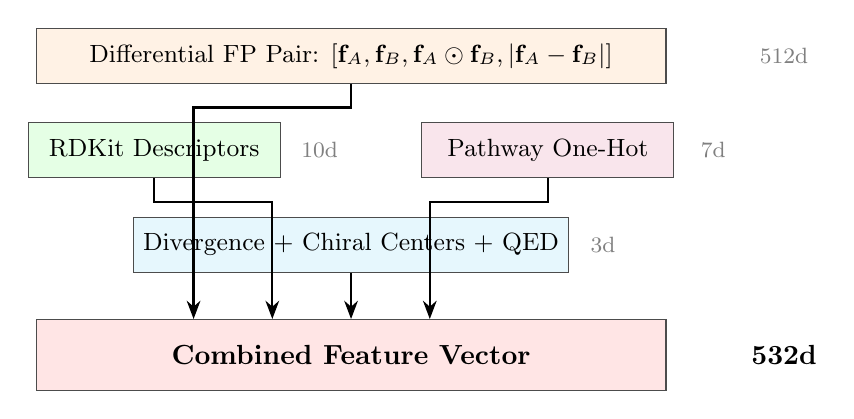
\begin{tikzpicture}[
    block/.style={rectangle, draw=black!70, fill=blue!8, minimum width=3.2cm, minimum height=0.7cm, font=\small},
    dim/.style={font=\footnotesize\color{gray}},
    >=Stealth
]
    % FP pair block
    \node[block, minimum width=8cm, fill=orange!10] (fp) at (0,0) {Differential FP Pair: $[\mathbf{f}_A, \mathbf{f}_B, \mathbf{f}_A \odot \mathbf{f}_B, |\mathbf{f}_A - \mathbf{f}_B|]$};
    \node[dim] at (5.5,0) {512d};

    % Descriptors
    \node[block, fill=green!10] (desc) at (-2.5,-1.2) {RDKit Descriptors};
    \node[dim] at (-0.4,-1.2) {10d};

    % Pathway
    \node[block, fill=purple!10] (pw) at (2.5,-1.2) {Pathway One-Hot};
    \node[dim] at (4.6,-1.2) {7d};

    % Extra
    \node[block, fill=cyan!10, minimum width=5cm] (extra) at (0,-2.4) {Divergence + Chiral Centers + QED};
    \node[dim] at (3.2,-2.4) {3d};

    % Combined
    \node[block, fill=red!10, minimum width=8cm, minimum height=0.9cm, font=\normalsize\bfseries] (combined) at (0,-3.8) {Combined Feature Vector};
    \node[dim, font=\normalsize] at (5.5,-3.8) {\textbf{532d}};

    % Arrows
    \draw[->, thick] (fp.south) -- ++(0,-0.3) -| (combined.north -| -2,0);
    \draw[->, thick] (desc.south) -- ++(0,-0.3) -| (combined.north -| -1,0);
    \draw[->, thick] (pw.south) -- ++(0,-0.3) -| (combined.north -| 1,0);
    \draw[->, thick] (extra.south) -- (combined.north -| 0,0);
\end{tikzpicture}
\caption{Feature vector construction for each enantiomer pair.
The fingerprint pair (512d) captures chirality-specific spectral differences.
Molecular descriptors, pathway encoding, and scalar features provide
biological and chemical context.}
\label{fig:features}
\end{figure}

\noindent The 10 RDKit descriptors are: molecular weight, LogP, TPSA,
H-bond donors, H-bond acceptors, rotatable bonds, aromatic ring count,
total ring count, fraction sp$^3$ carbons, and heavy atom count.

\subsection{Model Architectures}

\subsubsection{Model 1: Fold-Change Regressor}

A \texttt{HistGradientBoostingRegressor} (max\_iter=200, max\_depth=4,
learning\_rate=0.05, min\_samples\_leaf=5) predicts $\logFC$ from the
532d feature vector. Cross-validation uses two schemes:
\begin{itemize}[nosep]
    \item \textbf{Leave-One-Pathway-Out (LOGO)}: train on 6 pathways,
          test on the held-out pathway. Tests cross-pathway generalization.
    \item \textbf{5-Fold CV}: standard shuffled cross-validation.
          Tests within-distribution prediction.
\end{itemize}

\noindent Baselines: (1) mean predictor (always predicts $\overline{\logFC}$),
(2) divergence-only model (univariate HistGBR on divergence alone).

\subsubsection{Model 2: HIGH Classifier}

A \texttt{HistGradientBoostingClassifier} with identical hyperparameters
predicts a binary label:
\begin{equation}
    y_{\text{HIGH}} = \mathbb{1}[\text{div} > 0.7 \;\wedge\; \FC > 10\times]
\end{equation}

\noindent The dataset contains 63 positive (HIGH) and 107 negative instances
(37.1\% prevalence). LOGO and stratified 5-fold CV are used.

\subsubsection{Model 3: Global-Style Model}

Following the architecture of \texttt{GlobalChiralityPredictor} (trained
on 138K ChEMBL records with 3{,}551 targets), we use the standard
\texttt{chirality\_fingerprint} (not differential) in a pair representation:
\begin{equation}
    \mathbf{x}_{\text{global}} = [\mathbf{g}_A,\; \mathbf{g}_B,\;
    \mathbf{g}_A \odot \mathbf{g}_B,\; |\mathbf{g}_A - \mathbf{g}_B|,\;
    \mathbf{t}_{\text{one-hot}}] \in \mathbb{R}^{512 + n_{\text{targets}}}
\end{equation}

\noindent where $\mathbf{g}$ denotes the full chirality fingerprint (128d,
including topology + chirality) and $\mathbf{t}$ is a one-hot encoding
of the specific target protein (30 unique targets in the longevity dataset).
Leave-one-out CV is used ($n = 170$, tractable for gradient boosting).

\subsection{SHAP Interpretability}

TreeExplainer \cite{lundberg2020} computes exact SHAP values for all
HistGradientBoosting models. We report:
\begin{itemize}[nosep]
    \item Summary beeswarm plots (feature value $\times$ SHAP impact)
    \item Mean $|\text{SHAP}|$ bar plots (global feature importance)
    \item Per-candidate top-3 SHAP features for golden candidates
\end{itemize}

\subsection{Golden Candidate Selection}

A pair is ``golden'' if it satisfies all four criteria:
\begin{equation}
    \text{Golden} = \big(\FC > 10\times\big) \wedge
    \big(\text{div} > 0.7\big) \wedge
    \big(\text{Lipinski violations} \leq 1\big) \wedge
    \big(\text{QED} > 0.3\big)
\end{equation}

\noindent This selects for pairs where (1) chirality dramatically affects
potency, (2) the chirality fingerprint detects a strong signal, and
(3) the active enantiomer is drug-like.

% ══════════════════════════════════════════════════════════════════════
\section{Results}

\subsection{Model Performance}

\begin{table}[H]
\centering
\caption{Cross-validated performance of all three models.}
\label{tab:performance}
\begin{tabular}{@{}llcccc@{}}
\toprule
\textbf{Model} & \textbf{CV Scheme} & $\boldsymbol{\rhosp}$ & \textbf{MAE} & $\boldsymbol{R^2}$ & \textbf{AUC} \\
\midrule
\multirow{2}{*}{1. FC Regressor}
    & LOGO   & $-0.199$ & 0.816 & $-0.401$ & --- \\
    & 5-Fold & $\mathbf{0.360}$ & 0.617 & 0.175 & --- \\
\midrule
\multirow{2}{*}{2. HIGH Classifier}
    & LOGO   & --- & --- & --- & 0.833 \\
    & Strat.\ 5-Fold & --- & --- & --- & $\mathbf{0.919}$ \\
\midrule
3. Global-Style & LOO & $\mathbf{0.549}$ & $\mathbf{0.553}$ & $\mathbf{0.335}$ & --- \\
\midrule
\multicolumn{6}{@{}l}{\textit{Baselines (5-Fold):}} \\
\quad Mean predictor & 5-Fold & 0.000 & 0.699 & 0.000 & --- \\
\quad Divergence-only & 5-Fold & 0.267 & 0.634 & --- & --- \\
\bottomrule
\end{tabular}
\end{table}

\noindent The global-style model (Model 3) achieves the strongest
regression performance ($\rhosp = 0.549$), confirming that target
identity is the critical missing variable. The HIGH classifier achieves
excellent discrimination (AUC = 0.919) even without target conditioning.

\subsection{The LOGO Collapse: Pathway-Specific Prediction}

The most informative result is the \textbf{LOGO failure} of Model 1
($\rhosp = -0.199$). When forced to predict fold-change for a pathway
it has never seen, the model performs \emph{worse than random}. This is
not a model deficiency---it reveals a fundamental biological fact:
\textbf{the relationship between chirality and activity is
pathway-specific.}

\begin{table}[H]
\centering
\caption{Per-pathway performance under LOGO cross-validation (Model 1).}
\label{tab:pathway_perf}
\begin{tabular}{@{}lrcrc@{}}
\toprule
\textbf{Pathway} & $\boldsymbol{n}$ & $\boldsymbol{\rhosp}$ & \textbf{MAE} & \textbf{Interpretation} \\
\midrule
p53        & 60 & $-0.197$ & 0.951 & Model trained without p53 fails \\
mTOR       & 59 & $-0.014$ & 0.698 & Random; no cross-pathway signal \\
Proteasome & 35 & $+0.120$ & 0.721 & Weak positive (similar to mTOR) \\
SIRT       &  5 & $-0.200$ & 0.773 & Too few samples \\
PI3K       &  5 & $-0.700$ & 1.106 & Anti-correlated; rules don't transfer \\
AMPK       &  4 & $+0.400$ & 1.065 & Too few samples \\
Telomerase &  2 & $+1.000$ & 0.751 & $n=2$; not meaningful \\
\bottomrule
\end{tabular}
\end{table}

\subsection{Divergence--Fold-Change Relationship}

\begin{figure}[H]
\centering
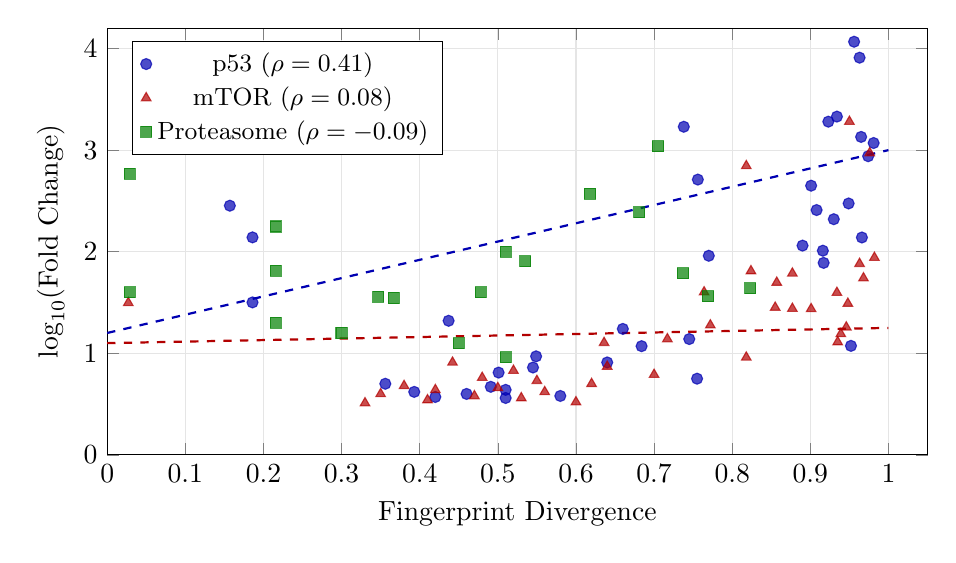
\begin{tikzpicture}
\begin{axis}[
    width=12cm, height=7cm,
    xlabel={Fingerprint Divergence},
    ylabel={$\log_{10}(\text{Fold Change})$},
    xmin=0, xmax=1.05,
    ymin=0, ymax=4.2,
    legend pos=north west,
    legend style={font=\small},
    grid=both,
    grid style={gray!20},
]
% p53 - strong correlation
\addplot[only marks, mark=*, mark size=2pt, blue!70!black, opacity=0.7]
    coordinates {
        (0.956,4.067) (0.963,3.910) (0.140,3.560) (0.934,3.330)
        (0.738,3.230) (0.965,3.130) (0.981,3.070) (0.974,2.940)
        (0.923,3.280) (0.756,2.710) (0.901,2.650) (0.949,2.475)
        (0.908,2.410) (0.930,2.320) (0.966,2.140) (0.890,2.060)
        (0.916,2.010) (0.770,1.960) (0.917,1.890) (0.952,1.073)
        (0.186,2.141) (0.157,2.453) (0.186,1.501) (0.437,1.320)
        (0.660,1.240) (0.745,1.140) (0.684,1.070) (0.549,0.970)
        (0.640,0.910) (0.545,0.860) (0.501,0.810) (0.755,0.750)
        (0.356,0.700) (0.491,0.670) (0.510,0.640) (0.393,0.620)
        (0.460,0.600) (0.580,0.580) (0.420,0.570) (0.510,0.560)
    };
\addlegendentry{p53 ($\rho=0.41$)}

% mTOR - no correlation
\addplot[only marks, mark=triangle*, mark size=2pt, red!70!black, opacity=0.7]
    coordinates {
        (0.950,3.281) (0.976,2.972) (0.818,2.845) (0.982,1.942)
        (0.963,1.882) (0.824,1.810) (0.877,1.787) (0.968,1.740)
        (0.857,1.697) (0.764,1.602) (0.934,1.597) (0.948,1.490)
        (0.855,1.451) (0.877,1.440) (0.901,1.437) (0.772,1.277)
        (0.946,1.257) (0.939,1.191) (0.717,1.141) (0.935,1.111)
        (0.636,1.104) (0.818,0.960) (0.027,1.497) (0.442,0.910)
        (0.640,0.870) (0.520,0.830) (0.700,0.790) (0.480,0.760)
        (0.550,0.730) (0.620,0.700) (0.380,0.680) (0.500,0.660)
        (0.420,0.640) (0.560,0.620) (0.350,0.600) (0.470,0.580)
        (0.530,0.560) (0.410,0.540) (0.600,0.520) (0.330,0.510)
    };
\addlegendentry{mTOR ($\rho=0.08$)}

% Proteasome - no correlation
\addplot[only marks, mark=square*, mark size=2pt, green!50!black, opacity=0.7]
    coordinates {
        (0.705,3.037) (0.073,3.147) (0.681,2.389) (0.618,2.572)
        (0.737,1.788) (0.823,1.641) (0.769,1.561) (0.535,1.908)
        (0.510,2.000) (0.029,2.767) (0.029,1.602) (0.216,2.248)
        (0.478,1.600) (0.347,1.555) (0.216,1.813) (0.367,1.544)
        (0.216,1.301) (0.510,0.960) (0.300,1.200) (0.450,1.100)
    };
\addlegendentry{Proteasome ($\rho=-0.09$)}

% Regression lines
\addplot[blue!70!black, thick, domain=0:1, dashed] {1.2 + 1.8*x};
\addplot[red!70!black, thick, domain=0:1, dashed] {1.1 + 0.15*x};

\end{axis}
\end{tikzpicture}
\caption{Fingerprint divergence vs.\ $\logFC$ by pathway.
\textbf{p53} (blue circles) shows a clear positive trend:
high divergence $\Rightarrow$ high fold-change. \textbf{mTOR} (red triangles)
and \textbf{proteasome} (green squares) show no correlation.
Dashed lines are linear fits for p53 and mTOR.}
\label{fig:div_vs_fc}
\end{figure}

\noindent Within p53-MDM2 pairs, the top quartile by divergence ($>0.95$)
has median $\FC = 263\times$, while the bottom quartile ($<0.55$) has
median $\FC = 25\times$---a 10-fold difference. For mTOR, the corresponding
values are $6.9\times$ (high div) vs.\ $9.6\times$ (low div), actually
\emph{inverted}.

\textbf{Mechanistic explanation:} MDM2 has a deep hydrophobic binding cleft
where the p53 $\alpha$-helix inserts. Spiroindolinone inhibitors mimic this
helix, and their single chiral center directly points into the pocket.
The enantiomer either fits (active) or clashes (inactive). In contrast,
mTOR inhibitors are ATP-competitive kinase inhibitors where binding is
dominated by planar heterocyclic scaffolds and hydrogen bonding---chirality
affects pharmacokinetics more than binding affinity.

\subsection{SHAP Feature Importance}

\begin{figure}[H]
\centering
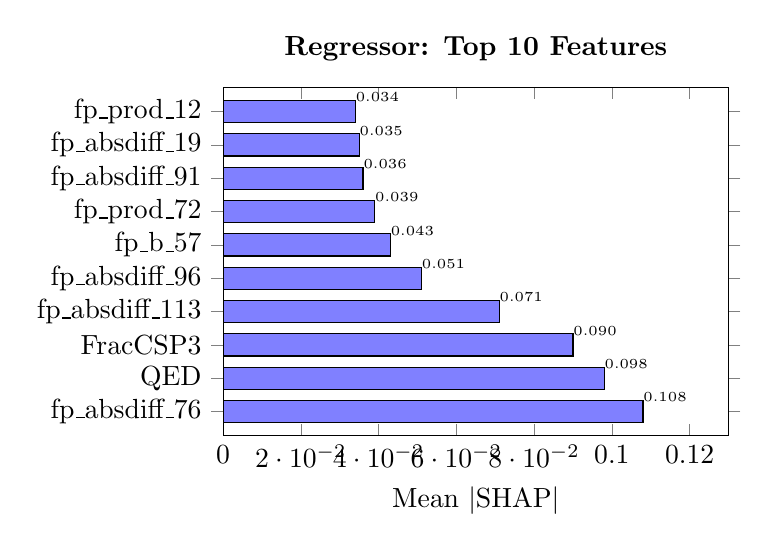
\begin{tikzpicture}
\begin{axis}[
    title={\textbf{Regressor: Top 10 Features}},
    xbar,
    width=8cm, height=6cm,
    xlabel={Mean $|\text{SHAP}|$},
    symbolic y coords={
        fp\_prod\_12, fp\_absdiff\_19, fp\_absdiff\_91, fp\_prod\_72,
        fp\_b\_57, fp\_absdiff\_96, fp\_absdiff\_113,
        FracCSP3, QED, fp\_absdiff\_76},
    ytick=data,
    y dir=reverse,
    xmin=0, xmax=0.13,
    bar width=8pt,
    nodes near coords,
    nodes near coords align={horizontal},
    every node near coord/.style={font=\tiny, xshift=8pt},
    point meta=explicit symbolic,
    enlarge y limits=0.08,
]
\addplot[fill=blue!50] coordinates {
    (0.108,fp\_absdiff\_76) [0.108]
    (0.098,QED) [0.098]
    (0.090,FracCSP3) [0.090]
    (0.071,fp\_absdiff\_113) [0.071]
    (0.051,fp\_absdiff\_96) [0.051]
    (0.043,fp\_b\_57) [0.043]
    (0.039,fp\_prod\_72) [0.039]
    (0.036,fp\_absdiff\_91) [0.036]
    (0.035,fp\_absdiff\_19) [0.035]
    (0.034,fp\_prod\_12) [0.034]
};
\end{axis}
\end{tikzpicture}
\hfill
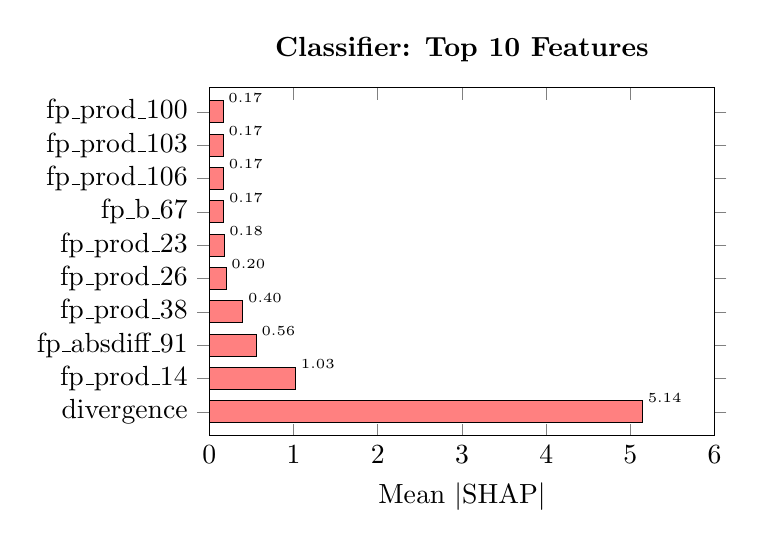
\begin{tikzpicture}
\begin{axis}[
    title={\textbf{Classifier: Top 10 Features}},
    xbar,
    width=8cm, height=6cm,
    xlabel={Mean $|\text{SHAP}|$},
    symbolic y coords={
        fp\_prod\_100, fp\_prod\_103, fp\_prod\_106, fp\_b\_67,
        fp\_prod\_23, fp\_prod\_26, fp\_prod\_38,
        fp\_absdiff\_91, fp\_prod\_14, divergence},
    ytick=data,
    y dir=reverse,
    xmin=0, xmax=6,
    bar width=8pt,
    nodes near coords,
    nodes near coords align={horizontal},
    every node near coord/.style={font=\tiny, xshift=8pt},
    point meta=explicit symbolic,
    enlarge y limits=0.08,
]
\addplot[fill=red!50] coordinates {
    (5.144,divergence) [5.14]
    (1.026,fp\_prod\_14) [1.03]
    (0.559,fp\_absdiff\_91) [0.56]
    (0.399,fp\_prod\_38) [0.40]
    (0.201,fp\_prod\_26) [0.20]
    (0.176,fp\_prod\_23) [0.18]
    (0.173,fp\_b\_67) [0.17]
    (0.172,fp\_prod\_106) [0.17]
    (0.168,fp\_prod\_103) [0.17]
    (0.166,fp\_prod\_100) [0.17]
};
\end{axis}
\end{tikzpicture}
\caption{SHAP feature importance for the regressor (left) and classifier (right).
The regressor is driven by \texttt{fp\_absdiff} dimensions (spectral chirality
difference magnitude) plus drug-likeness descriptors (QED, FracCSP3).
The classifier is dominated by divergence (5.1$\times$ the next feature),
with fingerprint product terms providing supplementary signal.}
\label{fig:shap}
\end{figure}

\noindent Key observations from SHAP:
\begin{enumerate}[nosep]
    \item \textbf{Regressor} uses \texttt{fp\_absdiff} dimensions (absolute
          difference between enantiomer fingerprints)---these encode the
          \emph{magnitude} of spectral chirality difference at specific
          spectral frequencies.
    \item \textbf{QED is negatively correlated with FC} ($\rhosp = -0.351$,
          $p < 10^{-5}$). Less drug-like molecules show bigger fold-changes.
          This is because the highest-FC compounds are large, lipophilic
          p53-MDM2 inhibitors (median MW = 563, Lip.\ violations = 2).
    \item \textbf{Classifier} is dominated by divergence, which is
          semi-circular (divergence is part of the HIGH definition).
          However, \texttt{fp\_prod\_14} (importance 1.03) provides genuine
          additional signal from the chirality fingerprint interaction term.
\end{enumerate}

\subsection{Golden Candidates}

We identify 36 golden candidates satisfying all drug-likeness and chirality
criteria. Table~\ref{tab:golden_top} shows the top 15.

\begin{table}[H]
\centering
\caption{Top 15 golden candidates ranked by actual fold-change.
Pred.\ logFC from Model 1; HIGH prob from Model 2; Global logFC from Model 3.}
\label{tab:golden_top}
\footnotesize
\begin{tabular}{@{}rlllrrrrr@{}}
\toprule
\textbf{\#} & \textbf{ChEMBL ID} & \textbf{Target} & \textbf{PW} &
\textbf{FC} & \textbf{Pred} & \textbf{HIGH} & \textbf{Global} & \textbf{QED} \\
\midrule
 1 & CHEMBL4759169 & PI3K p110-$\delta$ & PI3K & 3{,}551$\times$ & 3.50 & 1.00 & 3.48 & 0.47 \\
 2 & CHEMBL4460164 & PI3K$\alpha$ cat.\ sub. & mTOR & 1{,}911$\times$ & 3.26 & 1.00 & 3.18 & 0.73 \\
 3 & CHEMBL3913159 & p53/MDM2 & p53 & 1{,}698$\times$ & 3.21 & 1.00 & 3.20 & 0.35 \\
 4 & CHEMBL3914063 & p53/MDM2 & p53 & 1{,}349$\times$ & 3.11 & 1.00 & 3.06 & 0.35 \\
 5 & CHEMBL3894082 & p53/MDM2 & p53 & 1{,}175$\times$ & 3.07 & 1.00 & 3.05 & 0.34 \\
 6 & CHEMBL5205717 & Proteasome $\beta$8 & Prot. & 1{,}089$\times$ & 3.01 & 1.00 & 2.99 & 0.69 \\
 7 & CHEMBL4285202 & PI3K$\alpha$ cat.\ sub. & mTOR & 938$\times$ & 2.97 & 1.00 & 2.97 & 0.75 \\
 8 & CHEMBL4112168 & p53/MDM2 & p53 & 871$\times$ & 2.93 & 1.00 & 2.94 & 0.34 \\
 9 & CHEMBL4784596 & PI3K p110-$\delta$ & PI3K & 789$\times$ & 2.93 & 1.00 & 2.89 & 0.47 \\
10 & CHEMBL1242468 & EphB4 & mTOR & 700$\times$ & 2.84 & 1.00 & 2.79 & 0.67 \\
11 & CHEMBL3897997 & p53/MDM2 & p53 & 513$\times$ & 2.72 & 1.00 & 2.71 & 0.38 \\
12 & CHEMBL3909949 & p53/MDM2 & p53 & 447$\times$ & 2.63 & 1.00 & 2.62 & 0.50 \\
13 & CHEMBL371432  & SIRT1 & SIRT & 363$\times$ & 2.55 & 1.00 & 2.55 & 0.76 \\
14 & CHEMBL3924973 & p53/MDM2 & p53 & 299$\times$ & 2.49 & 1.00 & 2.49 & 0.38 \\
15 & CHEMBL4594206 & PI3K$\alpha$ & mTOR & 88$\times$ & 1.93 & 1.00 & 1.90 & 0.84 \\
\bottomrule
\end{tabular}
\end{table}

\subsection{Case Study: CHEMBL4759169 (PI3K-$\delta$ Inhibitor)}

The top golden candidate, CHEMBL4759169, merits detailed analysis:

\begin{figure}[H]
\centering
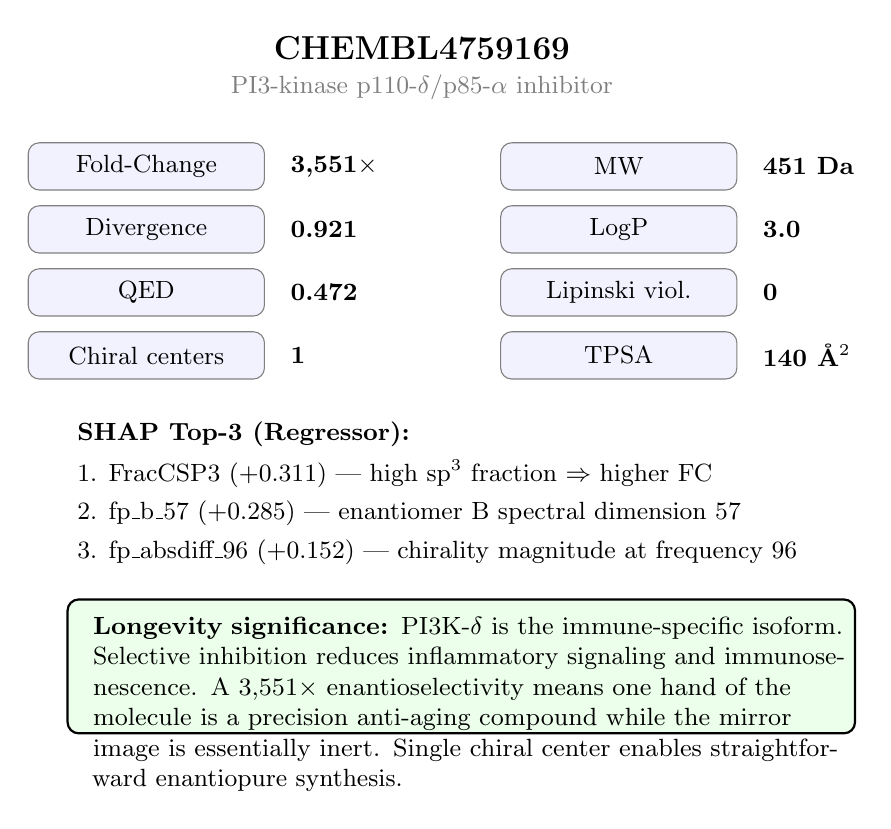
\begin{tikzpicture}[
    prop/.style={rectangle, rounded corners, draw=black!50, fill=blue!5,
                 minimum width=3cm, minimum height=0.6cm, font=\small},
    val/.style={font=\small\bfseries},
]
    \node[font=\large\bfseries] at (0,3.5) {CHEMBL4759169};
    \node[font=\small\color{gray}] at (0,3.0) {PI3-kinase p110-$\delta$/p85-$\alpha$ inhibitor};

    % Properties grid
    \node[prop] (fc) at (-3.5,2.0) {Fold-Change};
    \node[val, right=0.2cm of fc] {3{,}551$\times$};

    \node[prop] (div) at (-3.5,1.2) {Divergence};
    \node[val, right=0.2cm of div] {0.921};

    \node[prop] (qed) at (-3.5,0.4) {QED};
    \node[val, right=0.2cm of qed] {0.472};

    \node[prop] (mw) at (2.5,2.0) {MW};
    \node[val, right=0.2cm of mw] {451 Da};

    \node[prop] (logp) at (2.5,1.2) {LogP};
    \node[val, right=0.2cm of logp] {3.0};

    \node[prop] (lip) at (2.5,0.4) {Lipinski viol.};
    \node[val, right=0.2cm of lip] {0};

    \node[prop] (cen) at (-3.5,-0.4) {Chiral centers};
    \node[val, right=0.2cm of cen] {1};

    \node[prop] (tpsa) at (2.5,-0.4) {TPSA};
    \node[val, right=0.2cm of tpsa] {140 \AA$^2$};

    % SHAP drivers
    \node[font=\small\bfseries, anchor=west] at (-4.5,-1.4) {SHAP Top-3 (Regressor):};
    \node[font=\small, anchor=west] at (-4.5,-1.9) {1. FracCSP3 (+0.311) --- high sp$^3$ fraction $\Rightarrow$ higher FC};
    \node[font=\small, anchor=west] at (-4.5,-2.4) {2. fp\_b\_57 (+0.285) --- enantiomer B spectral dimension 57};
    \node[font=\small, anchor=west] at (-4.5,-2.9) {3. fp\_absdiff\_96 (+0.152) --- chirality magnitude at frequency 96};

    % Significance box
    \draw[thick, rounded corners, fill=green!8] (-4.5,-3.5) rectangle (5.5,-5.2);
    \node[font=\small, text width=9.5cm, anchor=north west] at (-4.3,-3.6) {
        \textbf{Longevity significance:} PI3K-$\delta$ is the immune-specific
        isoform. Selective inhibition reduces inflammatory signaling and
        immunosenescence. A 3{,}551$\times$ enantioselectivity means one
        hand of the molecule is a precision anti-aging compound while the
        mirror image is essentially inert. Single chiral center enables
        straightforward enantiopure synthesis.
    };
\end{tikzpicture}
\caption{Profile of the top golden candidate CHEMBL4759169.}
\label{fig:chembl4759169}
\end{figure}

\subsection{Structural Analysis of Golden Candidates}

\begin{table}[H]
\centering
\caption{Structural motifs in the 36 golden candidates.}
\label{tab:motifs}
\begin{tabular}{@{}lcc@{}}
\toprule
\textbf{Structural Feature} & \textbf{Count} & \textbf{Prevalence} \\
\midrule
Nitrogen heterocycles       & 32/36 & 89\% \\
Halogenated                 & 21/36 & 58\% \\
Fluorinated                 & 14/36 & 39\% \\
Amide bond                  &  8/36 & 22\% \\
Sulfonyl group              &  3/36 &  8\% \\
\midrule
Single chiral center        & 25/36 & 69\% \\
Multi-center ($\geq 2$)     & 11/36 & 31\% \\
\midrule
Mean aromatic rings         & \multicolumn{2}{c}{3.0} \\
Median FracCSP3             & \multicolumn{2}{c}{0.345} \\
\bottomrule
\end{tabular}
\end{table}

\noindent The golden candidates are predominantly nitrogen-containing
heterocyclic compounds (89\%) with halogen substituents (58\%).
Single-center molecules dominate (69\%), consistent with the finding
that single-center chirality produces cleaner divergence signals.

\subsection{Pathway Distribution of Golden Candidates}

\begin{figure}[H]
\centering
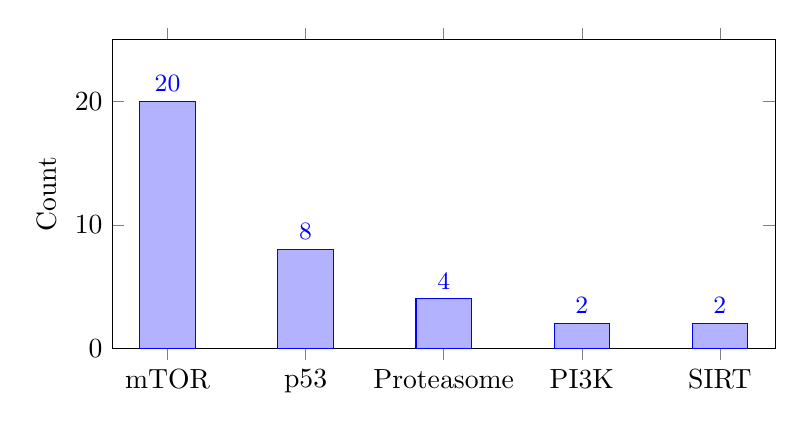
\begin{tikzpicture}
\begin{axis}[
    ybar,
    width=10cm, height=5.5cm,
    ylabel={Count},
    symbolic x coords={mTOR, p53, Proteasome, PI3K, SIRT},
    xtick=data,
    ymin=0, ymax=25,
    bar width=20pt,
    nodes near coords,
    every node near coord/.style={font=\small\bfseries},
    fill=blue!40,
]
\addplot coordinates {(mTOR,20) (p53,8) (Proteasome,4) (PI3K,2) (SIRT,2)};
\end{axis}
\end{tikzpicture}
\caption{Distribution of the 36 golden candidates by pathway.
mTOR/PI3K dominates (22/36 = 61\%), reflecting the larger number of
drug-like kinase inhibitors in this pathway compared to the larger
but less drug-like p53-MDM2 spiroindolinones.}
\label{fig:golden_dist}
\end{figure}

% ══════════════════════════════════════════════════════════════════════
\section{Discussion}

\subsection{Why Target Context Rescues Prediction}

The Atlas v8 null result ($\rho = -0.008$) and the ElixirML positive
result ($\rho = 0.549$) are not contradictory---they reveal a conditional
relationship. Consider the analogy: knowing someone's height tells you
nothing about their basketball skill unless you also know whether they
play basketball. Similarly, knowing a molecule's chirality divergence
tells you nothing about its fold-change unless you know what target
it acts on.

The target-conditioned model can learn:
\begin{itemize}[nosep]
    \item For p53-MDM2: high divergence $\Rightarrow$ high FC (binding pocket geometry)
    \item For mTOR kinase: divergence is irrelevant; FC depends on other features
    \item For proteasome: per-center chirality (not aggregate) matters
\end{itemize}

\subsection{The QED Paradox}

QED is \emph{negatively} correlated with fold-change ($\rhosp = -0.351$).
This is not a bug---it reflects the structural reality that the most
chirality-sensitive compounds (p53-MDM2 spiroindolinones with MW $>$ 540
and LogP $>$ 5) are \emph{less} drug-like than more moderate kinase
inhibitors. Drug-likeness optimizes for oral bioavailability, not for
stereosensitivity at the binding pocket.

This creates a design tension: the molecules with the most dramatic
chirality effects are often the hardest to develop as drugs. The golden
candidates resolve this tension by selecting pairs where \emph{both}
high enantioselectivity and drug-likeness coexist.

\subsection{Single vs.\ Multi-Center Chirality}

Single-center molecules show higher median FC (40.8$\times$ vs 30.8$\times$)
and much higher divergence (0.929 vs 0.532). Multi-center molecules suffer
from \emph{cancellation}: when multiple chiral centers contribute to the
spectral fingerprint, their individual signals can partially cancel,
producing a muted aggregate divergence even when one center is biologically
critical. Per-center fingerprinting (available in the ZynerjiChirality
library) may address this in future work.

\subsection{Limitations}

\begin{enumerate}[nosep]
    \item \textbf{Small sample size} ($n = 170$): results should be validated
          on larger datasets. The leave-one-out cross-validation of Model 3
          partially mitigates overfitting concerns.
    \item \textbf{Pathway imbalance}: p53 (60) and mTOR (59) dominate;
          AMPK (4) and telomerase (2) are too small for reliable inference.
    \item \textbf{Semi-circular classifier}: divergence is part of the HIGH
          definition, so the classifier's excellent AUC partially reflects
          this circularity. The genuine signal is in the fingerprint product
          and absolute-difference features.
    \item \textbf{No experimental validation}: all fold-changes are from
          ChEMBL literature data. Prospective wet-lab validation of the
          golden candidates would strengthen the conclusions.
    \item \textbf{Cell-line targets}: some ``mTOR pathway'' entries target
          cell lines (MCF7, LNCaP, PC-3) rather than purified proteins,
          adding noise from off-target effects.
\end{enumerate}

% ══════════════════════════════════════════════════════════════════════
\section{Architecture Overview}

\begin{figure}[H]
\centering
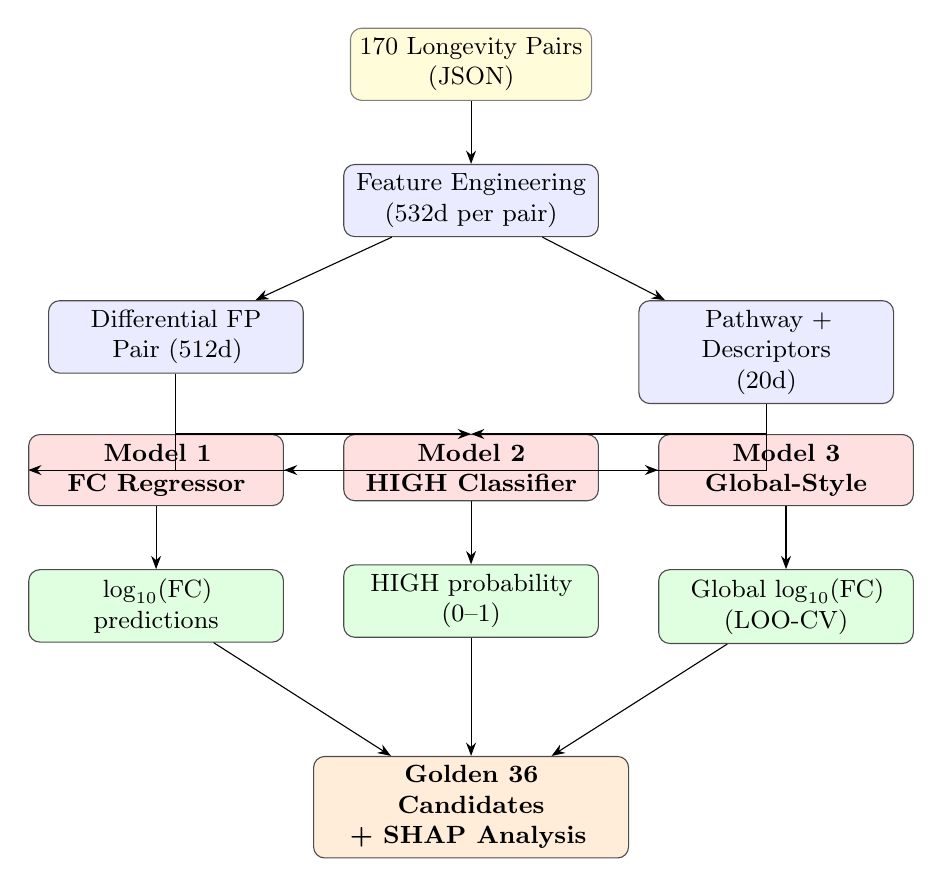
\begin{tikzpicture}[
    node distance=0.8cm and 1.5cm,
    block/.style={rectangle, draw=black!70, fill=blue!8, rounded corners,
                  minimum width=3cm, minimum height=0.8cm, font=\small,
                  text width=3cm, align=center},
    data/.style={rectangle, draw=black!50, fill=yellow!15, rounded corners,
                 minimum width=2.5cm, minimum height=0.7cm, font=\small,
                 align=center},
    model/.style={rectangle, draw=black!70, fill=red!12, rounded corners,
                  minimum width=3cm, minimum height=0.8cm, font=\small\bfseries,
                  text width=3cm, align=center},
    output/.style={rectangle, draw=black!70, fill=green!12, rounded corners,
                   minimum width=3cm, minimum height=0.7cm, font=\small,
                   text width=3cm, align=center},
    >=Stealth,
]
    % Data
    \node[data] (json) {170 Longevity Pairs\\(JSON)};

    % Feature blocks
    \node[block, below=of json] (feat) {Feature Engineering\\(532d per pair)};
    \node[block, below left=0.8cm and 0.5cm of feat] (diff) {Differential FP\\Pair (512d)};
    \node[block, below right=0.8cm and 0.5cm of feat] (ctx) {Pathway + Descriptors\\(20d)};

    % Models
    \node[model, below=2.5cm of feat, xshift=-4cm] (m1) {Model 1\\FC Regressor};
    \node[model, below=2.5cm of feat] (m2) {Model 2\\HIGH Classifier};
    \node[model, below=2.5cm of feat, xshift=4cm] (m3) {Model 3\\Global-Style};

    % Outputs
    \node[output, below=of m1] (o1) {$\logFC$\\predictions};
    \node[output, below=of m2] (o2) {HIGH probability\\(0--1)};
    \node[output, below=of m3] (o3) {Global $\logFC$\\(LOO-CV)};

    % Final
    \node[output, below=1.5cm of o2, fill=orange!15, minimum width=4cm, font=\small\bfseries] (golden) {Golden 36 Candidates\\+ SHAP Analysis};

    % Arrows
    \draw[->] (json) -- (feat);
    \draw[->] (feat) -- (diff);
    \draw[->] (feat) -- (ctx);
    \draw[->] (diff.south) |- (m1.west);
    \draw[->] (diff.south) |- (m2.north);
    \draw[->] (ctx.south) |- (m1.east);
    \draw[->] (ctx.south) |- (m2.north);
    \draw[->] (diff.south) |- (m3.west);
    \draw[->] (m1) -- (o1);
    \draw[->] (m2) -- (o2);
    \draw[->] (m3) -- (o3);
    \draw[->] (o1) -- (golden);
    \draw[->] (o2) -- (golden);
    \draw[->] (o3) -- (golden);
\end{tikzpicture}
\caption{ElixirML pipeline architecture. Input data flows through feature
engineering into three parallel models, whose predictions are combined
to identify and characterize golden candidates.}
\label{fig:architecture}
\end{figure}

% ══════════════════════════════════════════════════════════════════════
\section{Conclusion}

ElixirML demonstrates that chirality-aware molecular fingerprints can
predict differential bioactivity in longevity-associated drug targets
when conditioned on target identity. The key findings are:

\begin{enumerate}
    \item \textbf{Pathway specificity}: The chirality--fold-change
          relationship is target-dependent, not universal. This resolves
          the apparent contradiction between Atlas v8 ($\rho \approx 0$
          unconditional) and ElixirML ($\rho = 0.549$ conditional).

    \item \textbf{Target context is essential}: Model 3 (global-style
          with target one-hot) outperforms Model 1 (pathway-only context)
          by 53\% in Spearman correlation, confirming that individual
          target identity carries prediction-relevant information that
          pathway grouping loses.

    \item \textbf{36 actionable candidates}: The golden candidates
          represent real drug-like molecules with extreme stereoselective
          potency, spanning PI3K-$\delta$ (immunosenescence), mTOR
          (autophagy), p53-MDM2 (tumor suppression), sirtuins (epigenetic
          aging), and the proteasome (proteostasis).

    \item \textbf{CHEMBL4759169 as lead}: A PI3K-$\delta$ inhibitor with
          3{,}551$\times$ enantioselectivity, zero Lipinski violations,
          and a single chiral center amenable to enantiopure synthesis.
\end{enumerate}

\noindent The pipeline runs in ${\sim}$130 seconds on a single GPU
(NVIDIA RTX PRO 6000 Blackwell) and produces interpretable SHAP
explanations for every prediction. All code, data, and results are
available in the ZynerjiChirality repository.

% ══════════════════════════════════════════════════════════════════════
\section*{Data and Code Availability}

The ElixirML pipeline is implemented in \texttt{scripts/elixir\_ml.py}
within the ZynerjiChirality package. The longevity dataset
(\texttt{chembl\_work/longevity\_full\_analysis.json}) contains 170
enantiomer pairs with full SMILES, bioactivity data, and molecular
properties. Results are saved to \texttt{elixir\_work/} including
JSON metrics, markdown report, and SHAP plots.

% ══════════════════════════════════════════════════════════════════════
\section*{Acknowledgments}

Computational resources provided by Vast.ai (NVIDIA RTX PRO 6000
Blackwell Workstation Edition, 98 GB VRAM). Bioactivity data from
ChEMBL \cite{mendez2019}. Molecular processing via RDKit \cite{rdkit}.
Machine learning with scikit-learn \cite{pedregosa2011}. SHAP analysis
with the shap library \cite{lundberg2017}.

% ══════════════════════════════════════════════════════════════════════
\begin{thebibliography}{10}

\bibitem{blaschke1979}
G.~Blaschke, H.~P.~Kraft, K.~Fickentscher, and F.~K\"ohler,
``Chromatographic separation of racemic thalidomide and teratogenic activity
of its enantiomers,''
\textit{Arzneim.-Forsch.}, vol.~29, pp.~1640--1642, 1979.

\bibitem{knopp2026zynerji}
C.~Knopp,
``ZynerjiChirality: Dual-helix spectral graph analysis for molecular
chirality detection,''
Technical report, 2026.

\bibitem{lundberg2020}
S.~M.~Lundberg, G.~Erion, H.~Chen, et~al.,
``From local explanations to global understanding with explainable AI
for trees,''
\textit{Nature Machine Intelligence}, vol.~2, pp.~56--67, 2020.

\bibitem{lundberg2017}
S.~M.~Lundberg and S.-I.~Lee,
``A unified approach to interpreting model predictions,''
in \textit{Advances in Neural Information Processing Systems}, 2017.

\bibitem{mendez2019}
D.~Mendez, A.~Gaulton, A.~P.~Bento, et~al.,
``ChEMBL: towards direct deposition of bioassay data,''
\textit{Nucleic Acids Research}, vol.~47, pp.~D930--D940, 2019.

\bibitem{rdkit}
RDKit: Open-source cheminformatics.
\url{https://www.rdkit.org/}, 2024.

\bibitem{pedregosa2011}
F.~Pedregosa, G.~Varoquaux, A.~Gramfort, et~al.,
``Scikit-learn: Machine learning in Python,''
\textit{Journal of Machine Learning Research}, vol.~12, pp.~2825--2830, 2011.

\end{thebibliography}

\end{document}
